% \chapter{Results on Contribution to Classification of
% Complex Input Features \& Discussion}
% \label{chapter:results}
% \section{Introduction}


% \subsection{Discussion}

% \subsubsection{Comparison to other methods}

% A critical observation of recent post-hoc explanation methods is the tendency of certain methods, notably Layer-wise Relevance Propagation (LRP), Guided Backpropagation and GradCAM, to disproportionately emphasise the importance of edges in their heatmap representations. This propensity often leads to the overstatement of edges' relevance to the classification decision, potentially obscuring other crucial features. This phenomenon is not merely a visual artefact but a reflection of a deeper interpretative bias within these methods.

% This observation aligns with the findings of Adebayo et al.~\cite{AdebayoGMGHK18}, who noted that methods like Guided BackProp~\cite{SpringenbergDBR14} and GradCAM~\cite{ShrikumarGK17} demonstrate a lack of sensitivity to the network's final layers. This insensitivity suggests that these methods are inclined to highlight features such as objects and edges identified by the network's earlier layers, which might not be directly pertinent to the classification's final outcome. In contrast the \CTC\/ method is applied on the entire complex input features as found by the method defined in Chapter~\ref{chap:clustering}, which selects objects using Segment Anything Model (SAM). They are easier to understand, given humans naturally segment visual information into objects and the \CTC\/ method presents a single value of associated importance to each object. A user study was not conducted and remains a future work for this research (see Chapter~\ref{study}).

% The argument by~\cite{AdebayoGMGHK18} is further supported by the results presented in Figure~\ref{Fig:edges}, where LRP and Guided Backpropagation neglect background regions, which may be instrumental in the classification process. This oversight is particularly striking in cases where the background or less prominent features play a key role in the correct classification of the input. For example, in Figure~\ref{Fig:quality}, the bottom image is one of a Chimpanzee playing the piano. One can see that nearly all features (including the piano, a chair, ad other objects in the background) are highlighted by the majority of other methods --- leading the user to assume that nearly all features played a similar role in leading towards the classification. This might lead a user to also assume the network has simply memorised the input, rather than paying much attention to the Chimpanzee. However, this particular image is not part of the ILSVRC 2012 dataset~\cite{ILSVRC15} that the network has been trained on. In contrast \CTC\ presents an ordering of objects and features, and shows that despite the edges of a piano/chair appearing in generic heatmap methods, the most important feature, by several orders of magnitude is the Chimpanzee itself. This is a clear example of the value of \CTC\ in providing a more faithful explanation, and a more interpretable explanation.

% This point is perhaps better evidenced in situations of incorrect classification, as shown in Figure~\ref{Fig:edges}. All images have been incorrectly classified, however a generic heatmap does not offer a large amount of information as to \textit{why} this is the case. The tendency of generic heatmap methods to highlight edges and objects, rather than features, means that the user is left with little information as to why the network has made the wrong classification. In contrast, \CTC\ highlights features in the background, or indeed lend relevance to featureless (or edgeless) proportions of the image. An example of this is the background of the Truck/Moniter image in Figure~\ref{Fig:edges}, and on the image of a crib in Figure~\ref{Fig:quality}, which is considerably busy, however a major influence to the network (as found by \CTC) is the blanket. This is hard to spot in a generic heatmap, but the colouring of the blanket is clearly visible in the \CTC\ explanation. Indeed, the feature selection, along with clear ordering of the features provides the user with far clearer and informative explanations.

% While conventional methods often struggle to distinctly prioritise the significance of numerous overlapping or closely situated features, the \CTC\ method effectively highlights the most influential features in the classification process. It does so by aggregating and representing the collective importance of feature clusters, thus providing a streamlined and coherent interpretation. By simplifying the complexity inherent in feature-rich inputs, the \CTC\ method unveils the underlying patterns and relationships that may otherwise be obscured in a more granular or dispersed representation. The ability of the \CTC\ method to offer a clear ordering between features is invaluable, especially in scenarios where discerning the relative importance of features is crucial.



% \subsubsection{Comparison over different networks}



% \subsubsection{Comparison over Relevant Complex Input Features}

% A major influence on the quality of \CTC\ heatmaps is the method of feature selection. Most results presented in this chapter demonstrate the selection of masks selected based on size, as opposed to relevance. However, this introduces a bias towards larger features.

% Figure~\ref{Fig:small_parts} presents examples of mask selection by a relevance-based ordering. The author suggests this to be the method of choice when applied to complex images with multiple features, wherein the likely cause for a classification is a small, but highly relevant feature. For instance, the top-left hand image of a shoe-store shows a large amount of relevance for a single pair of shoes, which proportionally makes up a very small amount of a feature rich image.

% This is further demonstrated by a miss-classification. The second image at the top-left hand of Figure~\ref{Fig:small_parts} presents a photo of a tripod in a chapel, but VGG16 miss-classifies the image as a "swab". When choosing the most relevant complex input features a clear explanation is provided for where the mistake of the reasoning of the classifier lies. A feature selection method with a bias towards larger complex input features, is likely not to have identified this crucial element.

% However, this is not always the case. By selecting masks by relevance-based ordering, the shortcomings of other relevance metrics can negatively affect the performance of the \CTC\ explanation generated. For instance, the bottom left image in Figure~\ref{Fig:small_parts} fails to correctly identify the grass-hopper as the major feature in the image, instead showing a preference for smaller features which were attributed a high degree of relevance by the underlying attribution method (\LRP). The explanation in this case is still valid, as these small regions are assigned very low relevance, but it is not explaining which parts do contribute to the classifiers decision. The author suggest that in cases where the most relevant features do not provide an informative explanation the biggest complex input features may provide a better explanation.

% A key strength of the Contribution to Classification (CTC) method becomes apparent in scenarios where inputs possess a high density of features. The CTC method's unique ability to assign a singular relevance value to an entire cluster of features facilitates a clearer and more hierarchically structured interpretation of these features' importance. This aspect of the CTC method is particularly evident when analysing complex inputs, as seen in Figure~\ref{Fig:quality} and Figure~\ref{Fig:vgg19}.

% One of the most significant advantages of the Contribution to Classification (CTC) method is its capability to facilitate clear differentiation and ordered representation of features. This attribute is particularly crucial when analysing and contrasting the performance of different classifiers. In Figure~\ref{Fig:compare_models_same}, the same input is being processed by various networks, all of which correctly classify the input. Here, the figure not only showcases the classifications but also juxtaposes the explanations generated by the CTC method with those from other post-hoc interpretability methods, such as Input$\times$Gradient~\cite{SimonyanVZ13}, DeconvNet~\cite{ZeilerKTF10}, and Guided BackProp~\cite{SpringenbergDBR14}.

% In these figures, we observe inputs processed by the VGG16 model, characterised by their rich feature presence. Here, the CTC method shows its prowess, offering a stark contrast to traditional attribution methods. While conventional methods often struggle to distinctly prioritise the significance of numerous overlapping or closely situated features, the CTC method effectively highlights the most influential features in the classification process. It does so by aggregating and representing the collective importance of feature clusters, thus providing a streamlined and coherent interpretation.


% This clarity in feature prioritisation is not just a matter of visual neatness; it embodies a deeper understanding of the model's decision-making process. By simplifying the complexity inherent in feature-rich inputs, the CTC method unveils the underlying patterns and relationships that may otherwise be obscured in a more granular or dispersed representation. The ability of the CTC method to offer a clear ordering between features is invaluable, especially in scenarios where discerning the relative importance of features is crucial. This characteristic makes the CTC method particularly suited for applications in which a concise yet comprehensive overview of the model's reasoning is necessary.


% A critical observation of recent post-hoc explanation methods is the tendency of certain methods, notably Layer-wise Relevance Propagation (LRP), Guided Backpropagation and GradCAM, to disproportionately emphasise the importance of edges in their heatmap representations. This propensity often leads to the overstatement of edges' relevance to the classification decision, potentially obscuring other crucial features. This phenomenon is not merely a visual artefact but a reflection of a deeper interpretative bias within these methods.

% This observation aligns with the findings of Adebayo et al.~\cite{AdebayoGMGHK18}, who noted that methods like Guided BackProp~\cite{SpringenbergDBR14} and GradCAM~\cite{ShrikumarGK17} demonstrate a lack of sensitivity to the network's final layers. This insensitivity suggests that these methods are inclined to highlight features such as objects and edges identified by the network's earlier layers, which might not be directly pertinent to the classification's final outcome. This is further supported by the results presented in Figure~\ref{Fig:edges}, where LRP and Guided Backpropagation neglect background regions, which may be instrumental in the classification process. This oversight is particularly striking in cases where the background or less prominent features play a key role in the correct classification of the input.

% One of the most significant advantages of the Contribution to Classification (CTC) method is its capability to facilitate clear differentiation and ordered representation of features. This attribute is particularly crucial when analysing and contrasting the performance of different classifiers. In Figure~\ref{Fig:compare_models_same}, the same input is being processed by various networks, all of which correctly classify the input. Here, the figure not only showcases the classifications but also juxtaposes the explanations generated by the CTC method with those from other post-hoc interpretability methods, such as Input$\times$Gradient~\cite{SimonyanVZ13}, DeconvNet~\cite{ZeilerKTF10}, and Guided BackProp~\cite{SpringenbergDBR14}. A critical observation is that the explanations provided by these other methods show minimal variation across different networks, rendering it challenging to discern the distinct functional characteristics of each classifier. Furthermore, while LRP-$\alpha_1\beta_0$~\cite{bach2015pixel} generally produces similar explanations across different models, it notably struggles with networks like ResNet50. This inconsistency is likely attributable to the network’s unique structural features, such as residual connections, which impact the method's ability to generate clear explanations.

% In contrast to all other methods explanations, the CTC method's approach to feature ordering provides a more straightforward and insightful analysis. Its ability to distinctly outline and prioritise features makes it easier to identify and understand the differences in the functions learned by various classifiers. This advantage becomes even more pronounced in scenarios depicted in Figure~\ref{Fig:compare_models_not_same}, where inputs are not uniformly classified across all networks. In such cases, a robust interpretability method like CTC becomes invaluable. It aids in pinpointing differences in the learned functions between correctly and incorrectly classifying networks, offering critical insights into each model's decision-making process.

\newpage


% \section{Conclusion}


    % \item Throughout the results, images were included where the introduction of noise did not result in a change in the classification --- however, one can see that the average change in explanation was \textit{larger} than in comparison to a different type of noise

% \subsection{A meta-analysis of the experimental process}
% There are number of potential reasons why this is a shitty way of evaluating results.
% \begin{itemize}
%     \item Variance/sensitivity of metrics with respect to the size of the features being evaluated. E.g. in the case where there is already noise in the image? 
%     \item When does small noise turn into big noise -- what is the cut-off point where you'd like to see a big change in the explanation as opposed to a small change in the explanation? And how does this relate to the injection of noise? Would the injection of other features make more sense (is it still a ball player if there's an alien and a dog going heels-to-jesus in the background?)
%     \item Variance in the explanations with respect to the variance in the classification perhaps? 
%     \item Distance metrics --- there is some evidence to suggest that the traditional way of measuring distance between two explanations (traditional difference metrics) is not the best way of doing it. E.g. An increase in brightness might be a massive change in euclidean space, but in feature-space, this could be very small. 
%     \item Discussion over the differences between types of noise? We hvae noted that some networks are more sensitive to some types of noise than others. Why would this be the case? 
%     \item Discussion of computational cost in generating explanations? 
% \end{itemize}


% degree of input invariance between \CTC\ and Input$\times$Gradient, Integrated Gradients, DeconvNet, Guided BackProp, and LRP-$\alpha_1\beta_0$. The distance metric used to 


% The 















% employs a function to introduce uniform noise to the images. Unlike Gaussian noise, uniform noise affects all pixels with the same probability and intensity, making it a starkly different test for the attribution method's robustness. The noise is randomly generated within a specified range, which is -255 and 255 in the case of images. It is scaled by the intensity parameter, which suits as a noise level. The noise level can hold values between zero and one, where zero means no noise is added to the image and one means that the image is converted only to noise. The noise level parameter was set to 0.3 The result is then clipped to maintain valid pixel values.



% To asses the input invariance, saturation handling, and sensitivity of the \CTC\ method 

% The 
 

% The \CTC\ value of each complex feature is then found by propagating it through the network starting from the input layer until the classification is reached. We colour all the pixels that belong to each complex feature in one colour and then use that colour in the colour-coded legend next to the heatmap to show the \CTC\ value as a percentage of the overall classification. This deviates from traditional heatmaps, where seismic colours are used to show positive relevance with the intensity of red pixels, and negative relevance with the intensity of blue.
% \begin{figure}[t!]
% 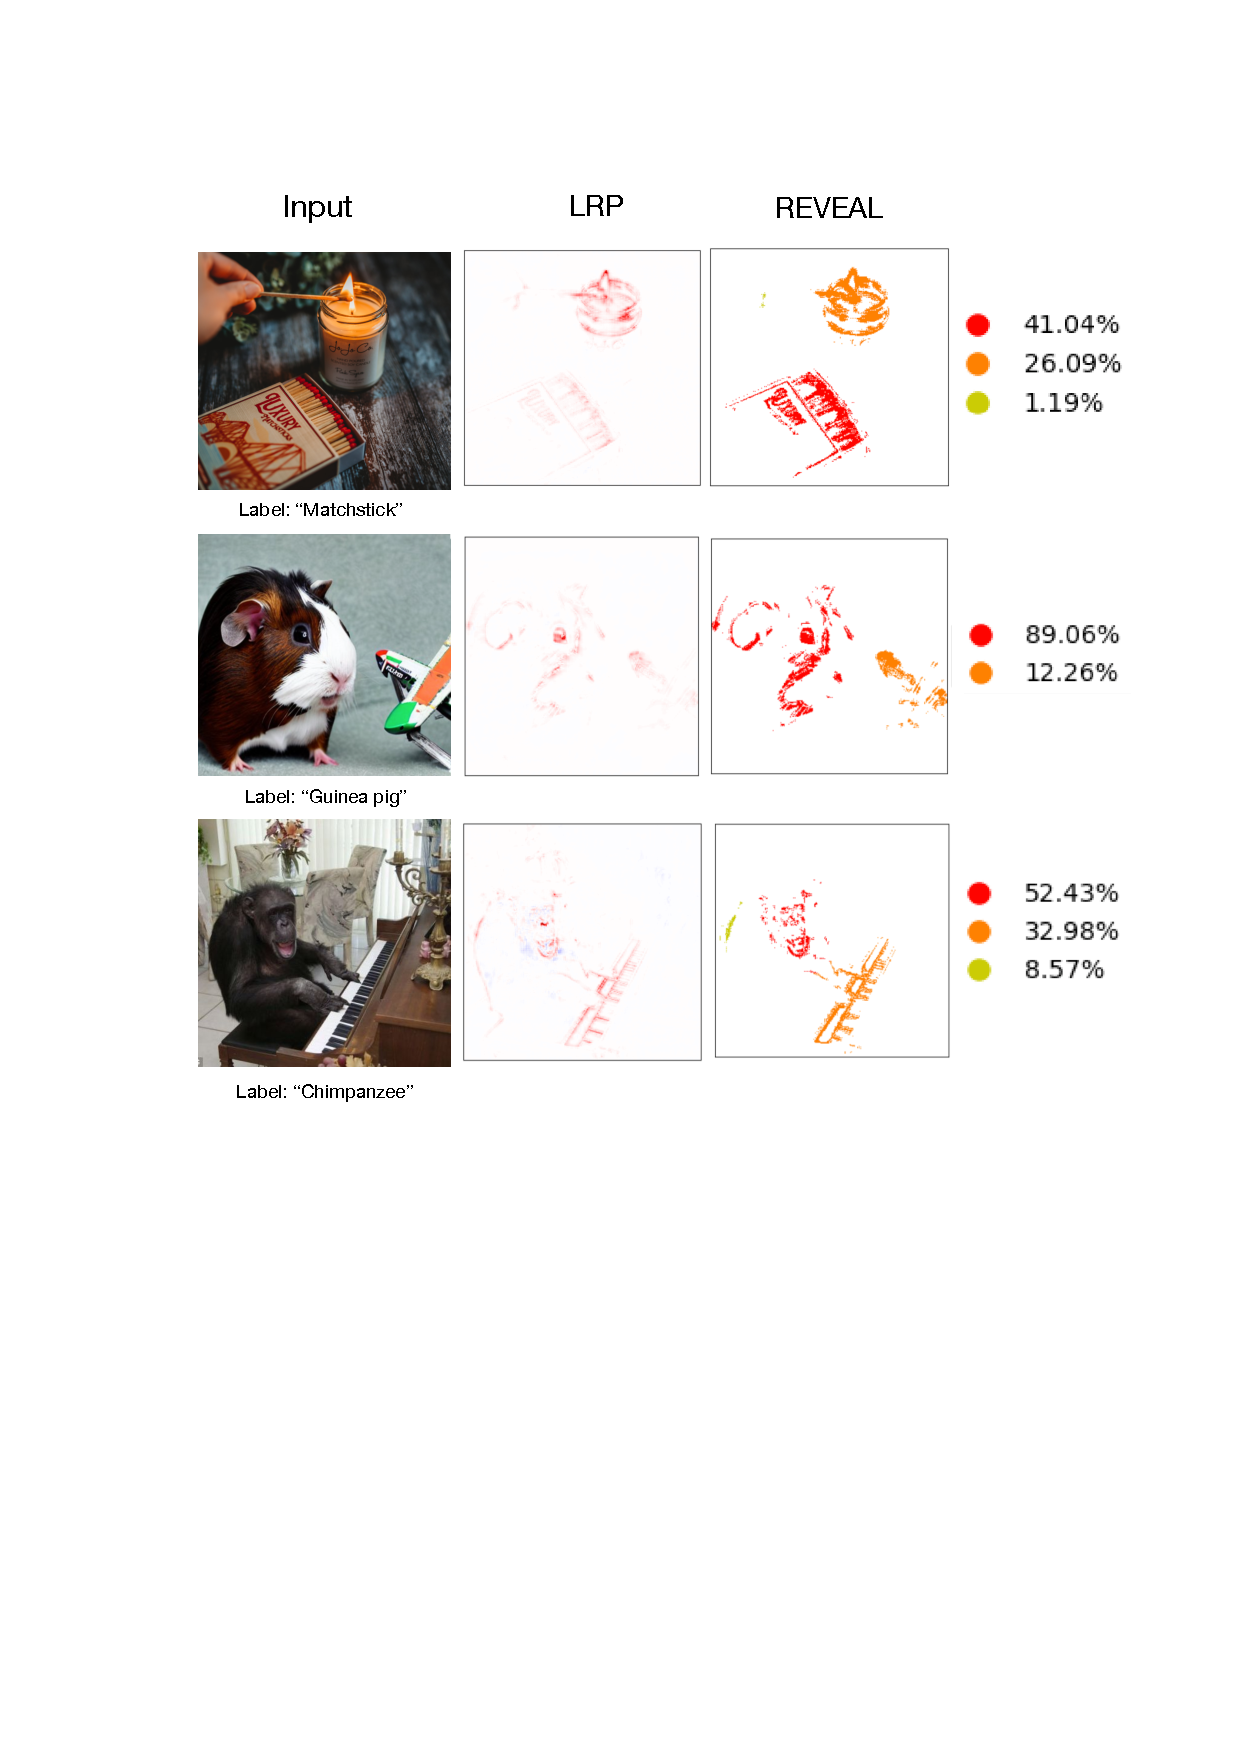
\includegraphics[width=\linewidth]{Chapters/Results/contribution_vs_relevance.pdf}
% 	\caption{Examples showcasing the difference between relevance and the \CTC\ value (contribution) of a feature.}
% 	\label{fig:differnce}
% \end{figure}
% % We argue that the single value of \CTC\ makes the comparison between different features easier. For example in Figure~\ref{fig:all}, when looking at \REVEAL\/'s explanation, each stocking (second row from the top) has a  \CTC\ value in isolation. One in particular (the central stocking) contributes far more than those on either side. This distinction cannot be drawn from any other technique and presents a visible difference even when each stocking is not clearly separated, as when clustering on top of \LRP\/. A similar phenomenon can be seen for the bottom plot of \ref{fig:all}, which is classified as a sports car, with the windscreen seemingly playing an equal part to the front wheel-arch and headlamp in all benchmarks when, in fact, the \CTC\ value is far greater for the wheel -- this is seen when detecting clusters on top of both Input$\times$Gradient and LRP-$\alpha_1\beta_0$.

% In Figure~\ref{fig:differnce} we show more examples that expose the difference between relevance and contribution. We have found that our technique is particularly useful when the input has features that are from two different classes that the network recognises. This brings back the point of relevance based techniques recognising edges that are relevant, but do not contribute much to the classification, as mentioned in section~\ref{subsection:contribution}. In the first example of Figure~\ref{fig:differnce} the classifier labels the input as matchsticks, \LRP\ finds both the matchsticks and the candle relevant, while putting more relevance on the candle. In contrast, \REVEAL\ shows that the matchsticks contribute more to the classification. This can also be seen in third example, where \LRP\ gives almost no relevance to the feature that contributes the most, as presented by \REVEAL\/.  

% The \CTC\ value as a percentage of the overall classification shows us how much of the classification can be explained by the feature alone. Note that the percentages don't total 100\%. As mentioned in Section~\ref{subsection:faithfulness}, this is intentional, as two distinct features may contribute to the same hidden neurons in the network and therefore have an overlapping contribution to the classification.

% As the clusters formed and evaluated by \REVEAL\ are concrete and have a single value of relevance, there is a far smaller chance of inconsistency of the interpretability. This property, as mentioned in section~\ref{subsection:contribution}, requires different users to comprehend the same information from a single explanation. While quantitative analysis is challenging as users find different explanations useful, \REVEAL\ is the only system that has predetermined and quantified complex features making it the only one that achieves that property. 
% \section{Conclusion}
